% Patch 0105: TikZ patterns. Uncoloured (form-only, with "pattern color") and the default black, over text and fills,
% as in the PaperA copy's timeline figure. Compare with Tectonic's PDF drawn by mutool.
\documentclass{article}
\usepackage{tikz}
\usetikzlibrary{patterns}
\pagestyle{empty}
\begin{document}
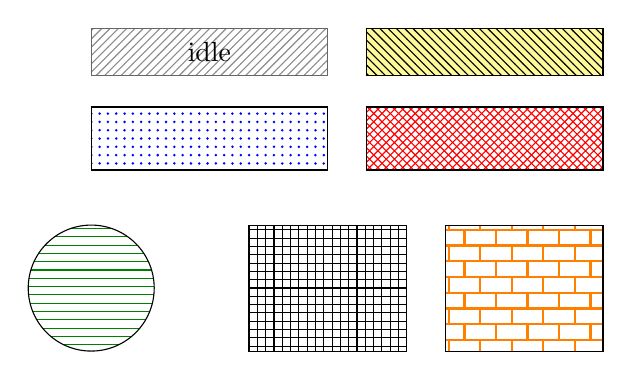
\begin{tikzpicture}
  \node[draw=black!60, line width=0.4pt, minimum width=3cm, minimum height=0.6cm,
        pattern=north east lines, pattern color=black!45] at (1.5,0) {idle};
  \fill[yellow!40] (3.5,-0.3) rectangle (6.5,0.3);
  \draw[pattern=north west lines] (3.5,-0.3) rectangle (6.5,0.3);
  \draw[pattern=dots, pattern color=blue] (0,-1.5) rectangle (3,-0.7);
  \draw[pattern=crosshatch, pattern color=red] (3.5,-1.5) rectangle (6.5,-0.7);
  \draw[pattern=horizontal lines, pattern color=green!50!black] (0,-3) circle (0.8);
  \draw[pattern=grid] (2,-3.8) rectangle (4,-2.2);
  \draw[pattern=bricks, pattern color=orange] (4.5,-3.8) rectangle (6.5,-2.2);
\end{tikzpicture}
\end{document}
